\clearpage
\Question{Tries}

Consider the following ternary search trie (TST):
\begin{center}
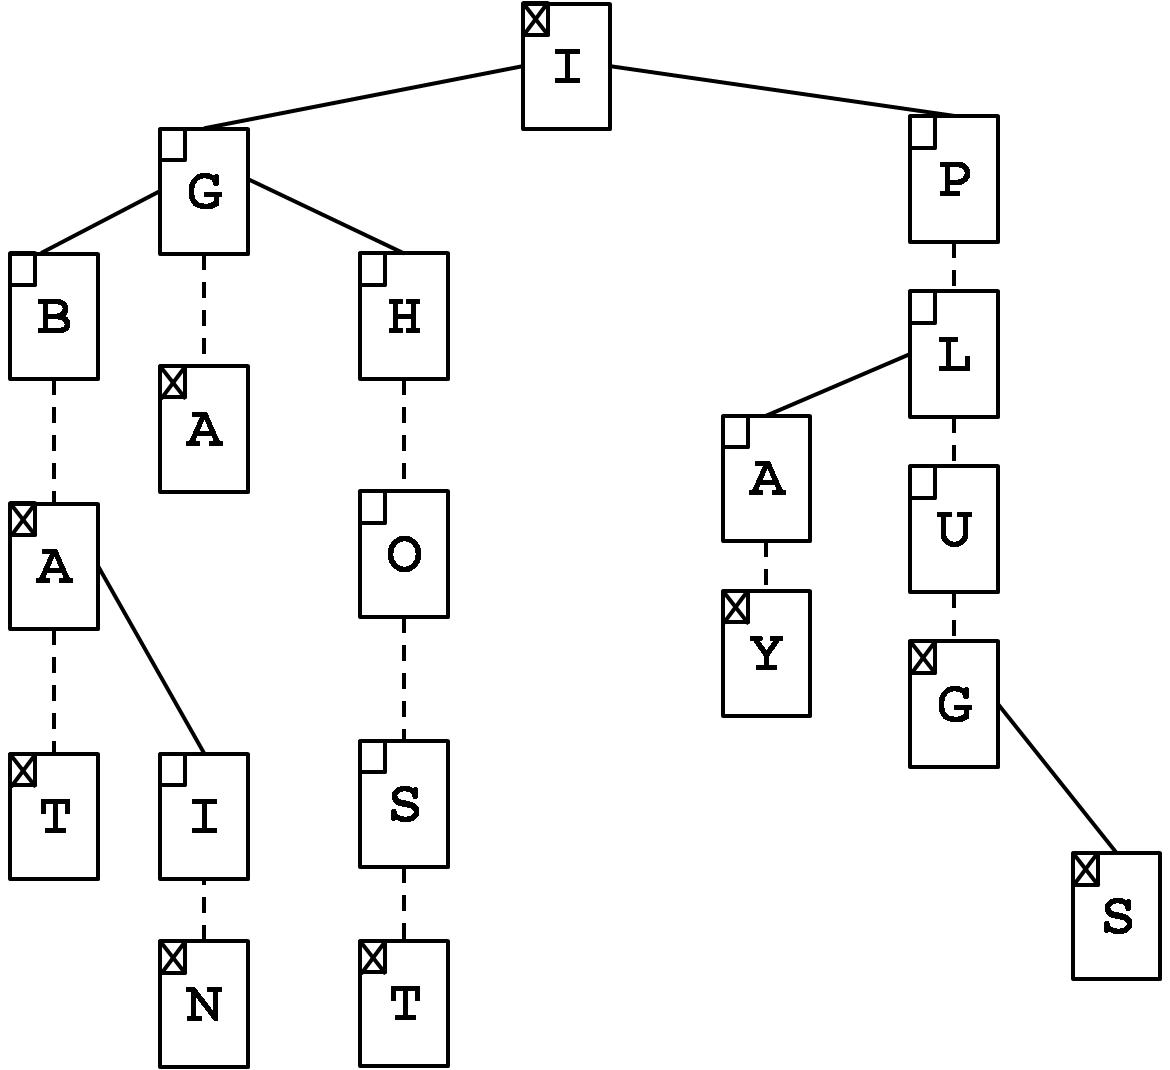
\includegraphics[width=.6\textwidth]{\img/tst1.png}
\end{center}

The dotted lines connect a node to its middle child, and
solid lines connect a node to its left and
right children.  An \emph{X} in the top left indicates that this
node ends a valid string.

%The lecture notes and accompanying code
%describe a desirable invariant of TSTs: that if the middle child is
%\lstinline'NULL', the node has to end a valid word. This TST does not have
%this invariant due to the topmost \lstinline'm' and \lstinline'e' nodes, but it
%is not a necessary invariant for safety or correctness. (The insertion
%and lookup algorithms work even without that invariant.)

\begin{parts}

\part[1]\TAGS{trie}
List all of the strings stored in the TST above, in alphabetical order.
\begin{framed}
\ifprintanswers{\color{\answerColor}
  BA, BAT, BIN, GA, HOST, I, PAY, PLUG, PLUS
}\else~\vspace{0.75in}\fi
\end{framed}

\RUBRIC
Part (a)
TAGS: trie

Gradescope rubric:  TODO

Commentary:
  BA, BAT, BIN, GA, HOST, I, PAY, PLUG, PLUS
  Half a point penalty if not alphabetical order
  Half point penalty for each missing/incorrect word
  Minimum of 0
ENDRUBRIC


\part[1]\TAGS{trie}
Add the words \lstinline'me', \lstinline'plugs', \lstinline'hope',
\lstinline'hot', \lstinline'top', and \lstinline'act' to the TST one
at a time, in the order given.  Do not worry about rebalancing.
\begin{framed}
\begin{lstlisting}[basicstyle=\basicstyle\color{\answerColor}]
           ----------i*-------
          /                   \
     ----g-----        ------- p
    /    |     \      /        |
  -b     a*     h    M     ----l
 / |            |    |    /    |
A  a*-          o    E*  a     u
|  |  \         |        |     |
C  t*  i     ---s        y*    g*--
|      |    /   |              |   \
T*     n*  P--  t*             S*    s*
           |  \
           E*  T*
\end{lstlisting}
\else~\vspace{7.0in}\fi
\end{framed}

\RUBRIC
Part (b)
TAGS: trie

Gradescope rubric:  TODO

Commentary:
  - Half point per missed or incorrect insertion until they hit 0
      - CT to the left of "ag"
      - PE to the left of "hos"
      - T to the right of "hop"
      - ME to the left of "r"
      - S below "plug"
  - Max 2 half-point penalties for screwed up Xes

(original TST in lowercase, additions in uppercase)
           ----------i*-------
          /                   \
     ----g-----        ------- p
    /    |     \      /        |
  -b     a*     h    M     ----l
 / |            |    |    /    |
A  a*-          o    E*  a     u
|  |  \         |        |     |
C  t*  i     ---s        y*    g*--
|      |    /   |              |   \
T*     n*  P--  t*             S*    s*
           |  \
           E*  T*
ENDRUBRIC

\end{parts}
